% Définitions
\card{définition}{DIAG}{%
  \begin{math}
    \{ <M> / <M>\:\not\in L(M) \}
  \end{math}
}

\card{définition}{EMPTY}{%
  \begin{math}
    \{ <M> / L(M) = \emptyset \}
  \end{math}
}

\card{définition}{HALT}{%
  \begin{math}
    \{ <M, w> /\:\text{M s'arrête sur l'entrée w} \}
  \end{math}
}

\card{définition}{UNIV}{%
  \begin{math}
    \{ <M, w> /\:w \in L(M) \}
  \end{math}
}

\card{définition}{Langage (Problème) décidable}{%
  Un langage L est dit \underline{décidable} s'il existe une machine de Turing M qui s'arrête sur toute entrée et telle que L = L(M).
}

\card{définition}{Langage (Problème) semi-décidable}{%
  Un langage L est dit \underline{semi-décidable} s'il existe une machine de Turing M telle que L = L(M).
}

\card{définition}{$\mathcal{D}, \mathcal{SD}, \mathcal{coSD}$}{%
  \begin{align*}
    \mathcal{D} &= \{ L /\:\text{L est décidable} \} \\
    \mathcal{SD} &= \{ L /\:\text{L est semi-décidable} \} \\
    \mathcal{COSD} &= \{ L /\:\text{$\overline{L}$ est semi-décidable} \}
  \end{align*}

  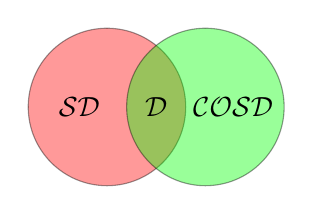
\begin{tikzpicture}
    \tikzset{venn circle/.style={draw,circle,minimum width=2cm,fill=#1,opacity=0.4}}

    \node [venn circle = red] (SD) at (0,0) {};
    \node [venn circle = green] (COSD) at (0:1.25cm) {};

    \node at (barycentric cs:SD=1/2,COSD=1/2 ) (D-endpoint) {$\mathcal{D}$};
    \node at ([xshift=-10pt]barycentric cs:SD=1/2 ) (SD-endpoint) {$\mathcal{SD}$};
    \node at ([xshift=+10pt]barycentric cs:COSD=1/2 ) (COSD-endpoint) {$\mathcal{COSD}$};
  \end{tikzpicture}
}


% Théorèmes
\card{théorème}{Théorème de Rice}{%
  Soit P une propriété non triviale de langage semi-décidable ($P \subset \mathcal{SD}, \neq \emptyset, \neq \mathcal{SD}$). \\
  Alors ${\{ <M> /\:L(M) \in P \}}$ est \underline{indécidable}.
}
